Initially, we present the statistical - and numerical methods used in the thesis. In addition, we introduce the necessary terminology and -theory from the study of dynamical systems to be able to construct our model.
\subsection{Stochastic Differential Equations}
First, we put forth the part from the general theory of stochastic differential equation that we need in order to derive estimators for the parameters of processes governed by them. 
\subsubsection{Itô integrals and - processes}
Broadly speaking a stochastic differential equation (SDE) is a generalization of a differential equation, where there is some term, which is a stochastic process. There exists many variants using different processes, yet we only consider processes driven by a Brownian motion - also known as a Wiener process. To define stochastic differential equations in this setting with more rigor we need to define a brownian motion: A brownian motion is a continuous stochastic processes, $W_t\in\mathbb{R}$ satisfying the following properties
\begin{enumerate}
    \item $X_0 = 0$ almost surely
    \item $\Delta W_n = W\left(t_{n + 1}\right) - W\left(t_{n}\right)\sim\mathcal{N}\left(0, t_{n + 1} - t_{n}\right)$
    \item $X_{t_1}\indep \left(X_{t_2} - X_{t_1}\right)\indep \dots \indep \left(X_{t_n} - X_{t_{n - 1}}\right), \: 0 < t_1 < t_2 < \dots < t_n$.
\end{enumerate}
This process is pivotal in the study of continuous-time stochastic processes. For our purposes, we define integration from $t_0$ to $t$ of some function $\sigma(X_t, t)$ with respect to $W_t$. We partition the interval $[t_0, t]$ into smaller intervals $[t_k, t_{k + 1}]$ with $t_0 \leq t_1 \leq \dots \leq t_n = t$. The integral is constructed by having the partition get increasingly finer
\begin{align}
    \int_{t_0}^t \sigma(X_s, s) \mathrm{d}W_s = \lim_{n \to \infty}\sum_{k = 0}^{n - 1} \sigma\left(X_{t_k}, t_k\right)\left(W_{t_{k + 1}} - W_{t_k}\right),\label{eq:itoIntegralDefinition}
\end{align}
where the limit is in $L_2$-sense \cite[equation 4.6]{Srkk2019}. \\
We call (\ref{eq:itoIntegralDefinition}) the Itô integral and it the central piece of Itô calculus; an area that expands the techniques of calculus to stochastic processes. Now to construct stochastic differential equations we write up the Itô integral equation
\begin{align}
    X_t - x_0 = \int_{t_0}^t b(X_s, s)\mathrm{d}s + \int_{t_0}^t \sigma(X_s, s)\mathrm{d}W_s. \label{eq:itoIntegralEquation}
\end{align}
Note that the first integral on the right hand side merely is a Riemann integral. A stochastic differential equation can then by understood by letting the limits of integration in (\ref{eq:itoIntegralEquation}) be $t$ and $t+\mathrm{d}t$ for some small $\mathrm{d}t$. That is as shorthand for (\ref{eq:itoIntegralEquation}) we may write
\begin{align}
    \mathrm{d}X_t = b(X_t, t)\mathrm{d}t + \sigma(X_t, t)\mathrm{d}W_t, \quad X_{t_0} = x_0 \label{eq:firstSDE},
\end{align}
and this is the general form of an SDE. \\
Although, the representation in (\ref{eq:firstSDE}) is the most common in the litterature and the one we use for the most part, we have to note that is merely a representation of (\ref{eq:itoIntegralEquation}). This can be seen, if we formally divide by $\mathrm{d}t$. We end up with a term, where we take the derivative of the Wiener process. This process has almost surely continuous sample paths, yet they are nowhere differentiable \cite[theorem 11.22 and theorem 11.35]{Hansen2022}.\\\\
To better understand stochastic differential equations we need to introduce a bit more nomenclature: The solution, $X_t$, is called an Itô process, and the values it can take is its state space. We refer to the functions $b(X_t, t)$ and $\sigma(X_t, t)$ as the drift- and diffusion coefficients respectively. For ease of language we sometimes leave out the "coefficient" part. In our applications the drift and diffusion depend on some parameter vector, $\theta\in\Theta\subseteq\mathbb{R}^p$. For typographical reasons though, we mostly suppress this dependence in the notation. Additionally, we say that the term with the diffusion coefficient is the noise term or stochastic term and the term with the drift is the deterministic term or deterministic part. The noise is additive, if the function $\sigma(X_t, t)$ is constant and multiplicative otherwise. Lastly, the stochastic differential equation has autonomous drift or diffusion, when they do not directly depend on time; the system as a whole is autonomous, if both parts are autonomous.\\
\\
Now, to motivate the arguably most important result in the study of stochastic differential equations, we evaluate the the Itô integral of the Wiener process
\begin{align}
    \int_0^t W_s \mathrm{d}W_s & = \lim_{n \to \infty}\sum_k W_{t_k}\left(W(t_{k + 1}) - W_{t_k}\right) \nonumber \\ 
    & = - \frac{1}{2}\lim_{n \to \infty}\sum_k \left(W(t_{k + 1}) - W(t_{k})\right)^2  + \frac{1}{2}\lim_{n \to \infty}\sum_k\left(W(t_{k + 1})^2 - W(t_{k})^2\right) \nonumber \\
    & = -\frac{t}{2} + \frac{W_t^2}{2}.
\end{align}
We have used the observation that the last sum was telescopic and equal to $W_t^2$. The first sum is the quadratic variation of the wiener process, which by \cite[theorem 11.34]{Hansen2022} is $t$.\\ Put differently, this means that
\begin{align}
    \mathrm{d}\left(\frac{1}{2}W_t^2\right) = W_t\mathrm{d}W_t + \frac{1}{2}\mathrm{d}t,
\end{align}
which is surprising, because it is not what we would expect from the normal chain rule. This means that Itô calculus needs its own version of the chain rule: Itô's formula \cite[Theorem 4.2]{Srkk2019}.  Given an Itô process, $X_t$, described by the SDE in (\ref{eq:firstSDE}) and a function $\varphi(X_t, t)$ of the process, then the Itô SDE for $\varphi$ can be computed by
\begin{align}
    \mathrm{d}\varphi(X_t, t) = \left(\frac{\partial \varphi}{\partial t} + \frac{\partial\varphi}{\partial x}b(X_t, t) + \frac{1}{2} \frac{\partial^2 \varphi}{\partial x^2}\sigma^2(X_t, t) \right)\mathrm{d}t + \frac{\partial\varphi}{\partial x}\sigma(X_t, t) \mathrm{d}W_t.
\end{align}
There are countless of important corollaries and applications of this result. The way we apply this result the most is qua the lamperti formation of a stochastic differential equation defined for an Itô process, $X_t$, given by (\ref{eq:firstSDE}) as
\begin{align}
    \psi(x, t) = \int_{\xi}^x \frac{\mathrm{d}u}{\sigma(u, t)}, \label{eq:firstLamperti}
\end{align}
for some $\xi$ in the state space of $X_t$. The lamperti-transform is obviously constructed such that $\mathrm{d}\psi(X_t, t)$ has additive noise, which is also easily verified with Itô's formula \cite[equation (7.5)]{Srkk2019}. We should be wary, though, as we have to ensure the transform is well-defined; we need to make sure we do not divide by zero in (\ref{eq:firstLamperti}). If we have a process, where this is ensured, it is called reducible. Further, to work with this in practice we define the transformed variable $Y_t := \psi(X_t, t)$; and to get the SDE in terms of $Y_t$, we thus need $\psi^{-1}$ to exist.\\\\
Finally, we note another result that is pivotal for the understanding of Itô processes. For fixed $t$, $X_t$ is a random variable, and we assume that it has some probability density, $p(X_t, t)$, with respect to the lebesgue measure. We do not work with explicitly, but it is worth mentioning that the variables are adapted to the filtration, $\mathcal{F}_n = \sigma\left(X_{t_i}: i \leq n\right)$. In addition, it each $X_t$ has some conditional density given by a previously observed variable $X_s$, $p(X_t, t | X_s, s), \; t\geq s$.\\ 
By \cite[theorem 7.1.2]{Oksendal2003_yu} all Itô processes are Markov processes, wherefore we need not information from the entire filtration, but just the information at the present, $X_s$, to characterize the transtion completely. The transition density of (\ref{eq:firstSDE}) is given by the following partial differential equation
\begin{align}
    \frac{\partial p(X_t, t | X_s, s)}{\partial t} = -\frac{\partial}{\partial x}\left(b(X_t, t)p(X_t, t | X_s, s)\right) + \frac{1}{2}\frac{\partial^2}{\partial x^2}\left(\sigma^2(X_t, t)p(X_t, t | X_s, s)\right),\label{eq:fokkerPlanck} 
\end{align}
with initial condition $p(x_t, t|x_s, s) = \delta(x_t - x_s)$ at time $t = s$ and where $\delta$ is the dirac delta function. We refer to this PDE as the Kolmogorov forward equation. As a result of giving us the transition density the Kolmogorov forward equation lets us calculate any conditional moment, if it exists. Additionaly, it allows us to derive score-function, defined as
\begin{align}
    U(\theta; X_t, t | X_s, s) = \frac{\partial}{\partial\theta}p(X_t, t | X_s, s), \label{eq:transitionScore}
\end{align}
and this can in principle be used to derive score equations for maximum likelihood estimation. In practice, however, (\ref{eq:fokkerPlanck}) is often untractable - meaning that we are unable to find the closed form solution for the transition density and thereby also the score. In this situation, one approach we often use is to somehow approximate the transition density.\\
Closely related to these concepts is the so-called infinitesemal generator 
\begin{align}
    \mathcal{L}\varphi(x) = b(x, t) \frac{\partial\varphi}{\partial x} + \frac{1}{2}\sigma^2(x, t)\frac{\partial^2\varphi}{\partial x^2} \label{eq:infinitesemalGeneratorDefinition},
\end{align}
which is an operator on some sufficiently regular function, $\varphi$. We say that $\varphi$ and $\lambda$ are the eigen functions and -values for the process respectively, if 
\begin{align}
    \mathcal{L}\varphi = -\lambda\varphi.
\end{align} 
These objects are central in the understanding of the evolution of the solutions to the stochastic differential equation, for which we do not have the closed form solutions to (\ref{eq:fokkerPlanck}). Under mild regularity conditions \cite[theorem 1.16]{StatisticalMethodsForSDE} namely states
\begin{align}
    \mathbb{E}\left[\varphi(X_{t}) \middle | X_{s}\right] = \exp\left(-\lambda \left(t - s\right)\right)\varphi \label{eq:momentConditions}, \quad t\geq s.
\end{align}
even when we cannot find the solution to (\ref{eq:fokkerPlanck}), we still have methods to calculate the conditional moments of the eigen functions of the process.\\
As is clear, though, we need the specific eigen function to be sufficiently simple e.g. a polynomium to actually be able to calculate the specific condtional moments, we are interested in. This is typically the first and second conditional moment.
\subsubsection{The Ornstein-Uhlenbeck process}
As mentioned, closed-form solutions can only be derived for select stochastic differential equations. One such process is the Ornstein-Uhlenbeck process
\begin{align}
    \mathrm{d}X_t = -\alpha_0\left(X_t - \mu\right)\mathrm{d}t + \sigma \mathrm{d}W_t, \quad X_{t_0} = x_0. \label{eq:originalOUprocess}
\end{align}
In this rather simple process the drift and diffusion are parameterized by $\theta = \left(\alpha_0, \mu, \sigma\right)^\top$ with the constraint that $\alpha_0, \sigma>0$.
To get the closed form solution for this SDE multiply (\ref{eq:originalOUprocess}) with $\exp\left(\alpha_0 t\right)$ and rearrange
\begin{align}
    \exp\left(\alpha_0 t\right)\mathrm{d}X_t + \exp\left(\alpha_0 t\right) \alpha_0 X_t \mathrm{d}t = \exp\left(\alpha_0 t\right)\alpha_0\mu \mathrm{d}t + \exp\left(\alpha_0 t\right)\sigma \mathrm{d}W_t
\end{align}
Use Itô's formula on $\exp\left(\alpha_0 t\right)X_t$ to see
\begin{align}
    \mathrm{d}\left(\exp\left(\alpha_0 t\right)X_t\right) &= \exp\left(\alpha_0 t\right)\alpha_0 \mu \mathrm{d}t + \exp\left(\alpha_0 t\right) \sigma \mathrm{d}W_t \nonumber
\end{align}
Understanding this as the integral equation (\ref{eq:itoIntegralEquation}) yields
\begin{align}
    \exp\left(\alpha_0 t\right)&X_t - \exp\left(\alpha_0 t_0\right)x_0 = \left(\exp\left(\alpha_0 t\right) - \exp\left(\alpha_0 t_0\right)\right)\mu + \int_{t_0}^t \exp\left(\alpha_0 s\right)\sigma \mathrm{d}W_s \nonumber \\
    &X_t = \exp\left(-\alpha_0\left(t - t_0\right)\right)\left(x_0 - \mu\right) + \mu + \int_{t_0}^t \exp\left(-\alpha_0 \left(t - s\right)\right)\sigma \mathrm{d}W_s \label{eq:OU_solution},
\end{align}
which was what we wanted. Now, since the increments of the brownian motion is gaussian, the solution $X_t$ for given $t$ is gaussian. We can easily find its mean and variance using the following properties of the Itô integral \cite[theorem 3.2.1 and lemma 3.1.5]{Oksendal2003_yu}
\begin{align}
    \mathbb{E}\left[\int_{t_0}^t f(X_s, s) \mathrm{d}W_s\right] &= 0 \label{eq:meanOfItoIntegral},\\
    \mathbb{E}\left[\left(\int_{t_0}^t f(X_s, s) \mathrm{d}W_s\right)^2\right] &= \int_{t_0}^t \mathbb{E}\left[\left(f(X_s, s)\right)^2\right] \mathrm{d}s. \label{eq:ItoIsometry}
\end{align}
Taking expectation of (\ref{eq:OU_solution}) and using (\ref{eq:meanOfItoIntegral}) we get
\begin{align}
    \mathbb{E}\left[X_t\right] = \exp\left(-\alpha_0\left(t - t_0\right)\right)\left(x_0 - \mu\right) + \mu. \label{eq:OU_mean}
\end{align}
Then we take the variance of (\ref{eq:OU_solution})
\begin{align}
    \mathrm{Var}\left[X_t\right] &= \sigma^2\mathrm{Var}\left[\int_{t_0}^t \exp\left(-\alpha_0 \left(t - s\right)\right)\sigma \mathrm{d}W_s\right],\nonumber \\
    & = \sigma^2\left(\int_{t_0}^t \mathbb{E}\left[\exp\left(-2\alpha_0\left(t - s\right)\right)\right] \mathrm{d}s + 0^2 \right), \nonumber \\
    & = \frac{\sigma^2}{2\alpha_0}\left(1 - \exp\left(-2\alpha_0(t - t_0)\right)\right). \label{eq:OU_variance}
\end{align}
Where we use both (\ref{eq:meanOfItoIntegral}) and (\ref{eq:ItoIsometry}) in the second step. Note that $\alpha_0 > 0$, we see that (\ref{eq:meanOfItoIntegral}) goes to $\mu$, when $t$ goes to $\infty$. This phenomenon is called mean-reverting. There are a lot of other Itô process that have this property; and as we will see, it stems from the structure of the drift. Also, for the same reasons (\ref{eq:OU_variance}) goes to $\frac{\sigma^2}{2\alpha_0}$.
\subsubsection{Pearson diffusions}
A special family of one-dimensional Itô processes are the Pearson diffusions. Structurally, they are very similiar to the Ornstein-Uhlenbeck process in the way that they share drift function; as we will see this means that they are mean-reverting as well. More specifically, we define a pearson diffusion as a solution to a stochastic differential equation on the form
\begin{align}
    \mathrm{d}X_t = -\alpha_0 \left(X_t - \mu\right)\mathrm{d}t + \sigma\sqrt{\left(aX_t^2 + bX_t + c\right)}\mathrm{d}W_t, \: \alpha_0, \sigma > 0. \label{eq:pearsonDiffusion}
\end{align}
For appropriate choices of $a, b, c$ making the square-root well-defined in the state space of $X_t$. Our focus is on the ergodic pearson diffusions; one can show that this is a class of six special diffusions \cite[p.36]{StatisticalMethodsForSDE}. \\
Amongst other things, we consider the Lamperti-transform defined in (\ref{eq:firstLamperti}). Here, it is
\begin{align}
    Y_t := \psi\left(X_t, t\right) = \int_{\xi}^{X_t} \frac{\mathrm{d}x}{\sqrt{\left(ax^2 + bx + c\right)}}. \label{eq:lampertiDefinition}
\end{align}
Again, for some appropriate $\xi$ in the state space of the respective processes. To see that $\mathrm{d}\psi\left(X_t, t\right)$ has additive noise, we present the its SDE, derived using Itô's formula
\begin{align}
    \mathrm{d}\psi\left(X_t, t\right) = - \frac{1}{\sqrt{\left(aX_t^2 + bX_t + c\right)}}\left(\alpha_0\left(X_t - \mu\right) + \frac{\sigma^2}{4}\left(2aX_t + b\right)\right)\mathrm{d}t + \sigma \mathrm{d}W_t.
\end{align}\\
However, to get the expression of $\mathrm{d}Y_t$ we have to invert $\psi\left(X_t, t\right)$ and this is obviously not possible in the general case of (\ref{eq:lampertiDefinition}); it needs to be handled casewise.\\
We sketch a quick overview of the processes \cite[p.36]{StatisticalMethodsForSDE} and their lamperti-transform\\\\
\begin{table}[h!]
    \begin{center}
    \begin{tabular}{lllll}\hline
    \textbf{Name} & \textbf{Diffusion term} & \textbf{Lamperti-transform} & \textbf{State space}\\ \hline
    Ornstein-Uhlenbeck  & $\sigma$  & $X_t$ & $\mathbb{R}$ \\
    Square-root process & $\sigma\sqrt{X_t}$  & $ 2\sqrt{X_t}$ & $\mathbb{R}_{>0}$ \\
    Mean-reverting GBM  & $\sigma X_t $  & $ \log\left(X_t\right)$  & $\mathbb{R}_{>0}$ \\
    Skew t-diffusion  & $\sigma\sqrt{X_t^2 + 1}$  & $ \sinh^{-1}(X_t)$ & $\mathbb{R}$\\
    Scaled F-diffusion  & $\sigma\sqrt{X_t\left(X_t + 1\right)}$  & $ 2\sinh^{-1}\left(\sqrt{X_t}\right)$ & $\mathbb{R}_{>0}$ \\
    Jacobi-diffusion  & $\sigma\sqrt{X_t\left(1 - X_t\right)}$  & $ 2\sin^{-1}\left(\sqrt{X_t}\right)$ & $(0, 1)$ \\ \hline
    \end{tabular}
    \caption{Overview of the ergodic pearson diffusions}
    \label{table:ergodicDiffusions}
\end{center}
\end{table}\\
For the the expressions of $\mathrm{d}Y_t$ for each of the diffusions refer to appendix \ref{sec:AppendixEstim}. If we consider the diffusion terms in table \ref{table:ergodicDiffusions}, it is clear that (\ref{eq:lampertiDefinition}) is always well-defined; that is, the processes are reducible. Additionally, we see that the respective lamperti-transform are one-to-one on the state space and therefore have well-defined inverse. \\\\
In spite of not being specifically important for our purposes, we note that although named the erdogic pearson diffusions, some are not ergodic for any choice of parameters. Whether there are any conditions for ergodicity and what these are depends on the diffusion in question; the condition, of course, is on the parameters. For instance, the Ornstein-Uhlenbeck is always ergodic and has invariant distribution $\mathcal{N}\left(\mu, \frac{\sigma^2}{2\alpha_0}\right)$, whereas the square-root process is ergodic if and only if $2\alpha_0\mu\geq \sigma^2$ with invariant distribution $\Gamma\left(\frac{2\alpha_0\mu}{\sigma^2}, \frac{2\alpha_0}{\sigma^2}\right)$. \\
Yet, more beneficial for our applications is the fact that Forman and Sorensen \cite{FormanSorensen2008} proved that for our ergodic diffusions, the eigen functions are all polynomials. Because of this, we can use (\ref{eq:momentConditions}) to derive any conditional moment of these processes, in spite of the fact that the transition densities themselves, for the most part, are unknown. Still, the calculations can become quite involved algebraically; this is especially true for moments of higher order. For this reason, we only used the first two eigenfunctions and eigenvalues: those associated with the first- and second-order polynomials. To this end, observe that regardless of the noise term, (\ref{eq:pearsonDiffusion}) always have the same first-order eigen function and eigen value, due to the vanishing of the noise term in (\ref{eq:infinitesemalGeneratorDefinition}), whenever $\varphi$ is affine. This naturally results in the same conditional mean too, which for any of the diffusions in table \ref{table:ergodicDiffusions} is
\begin{align}
    \mathbb{E}\left[X_{t_{i}+\Delta} \middle|X_{t_{i}} \right] = \exp\left(-\alpha_0\Delta t\right)\left(x-\mu\right) + \mu
\end{align}
This we also verify directly for a concrete pearson diffusion in (\ref{eq:directVerificationCondMean}). Though, it is evident that the calculations are completely analagous for the other pearson diffusions. We regognize the mean-reverting nature of the conditional moments that the moment of the OU-process had. With regard to the the conditional second moments and -variances, however, we need to consider the processes individually.
\subsubsection{Discretization of stochastic differential equations}
In their abstract form stochastic differential equation are inherently different to the actual observations from them in real world applications.
When sampling or considering sample paths from stochastic differential equations we are naturally limited to a finite amount of samples. Typically, we are in a situation, where we have samples $X_{t_0},\dots,X_{t_n}$ for some times $t_0,\dots,t_n$. We denote the time between the observations the temporal resolution of the data write $\Delta t_i = t_{i} - t_{i - 1}$; this quantity is for simplicity often constant and when it is, we refer to it as uniform temporal resolution. Given the sample from data, we can just use the markov property and the methods that stem for it, to do inference. If we on the other hand, want to draw samples from an SDE such as  (\ref{eq:firstSDE}), we need to use a different idea. 
\subsection{Dynamical systems}
When studying a system that evolves over time, one thing that frequently interests us is the long-term behaviour of the system: Will it reach an equillibrium of sorts, oscillate or something completely different. The answers to this question are the systems dynamics, and the type we are concerned with are the differential equation type of dynamical systems. Initially, we introduce relevant terminology for dynamical systems in their classic deterministic setting; then we see that they also align well in the setting of stochastic differential equation. 
\subsubsection{Deterministic Dynamical Systems and bifurcations}
A general dynamical system can be written as
\begin{align}
    \mathrm{d}x_t = f(x_t, \lambda)\mathrm{d}t, \label{eq:generalDynamicalSystem}
\end{align}
where $x_t$ is some variable of interest and $\lambda$ is some parameter that, for now, is fixed. We are often interested in the flow of the system. More specifically, we say that the flow is to the right, when (\ref{eq:generalDynamicalSystem}) is positive and to the left, if it negative. In the case, when $f(x_0, \lambda) = 0$, the point $x_0$ is called a fixed point. The fixed point is stable, if $\frac{\partial}{\partial x}f(x_0, \lambda) < 0$ and unstable, if it is positive. As an example consider the double-well potential given by the differential equation 
\begin{align}
    \mathrm{d}x_t = f_{DW}(x_t, \lambda) = \left(-x_t^3 - \lambda x_t\right) \mathrm{d}t \label{eq:originalDW}
\end{align}
The fixed points for (\ref{eq:originalDW}) are found by 
\begin{align}
    f_{DW}(x, \lambda) = x\left(-x^2 - \lambda\right) = 0,
\end{align}
clearly $x_0 = 0 \lor x_0 = \pm \sqrt{-\lambda}$. As 
\begin{align}
    \frac{\partial}{\partial x}f_{DW}(x, \lambda) = -3x^2 - \lambda,
\end{align}
we see that the fixed point located at zero, is unstable for $\lambda<0$ and stable when $\lambda>0$. For the other fixed points, direct calculations show $\frac{\partial}{\partial x}f_{DW}(x_0, \lambda) = 2\lambda$. These fixed points, however, only exist for negative $\lambda$, for which they clearly are stable. 
Perhaps a bit surprisingly, a more often utilized approach for these kinds of problems is a rather qualitative one. As an example, we could achieve the same results by graphing the differential equation
\begin{figure}[h]
    \begin{center}
        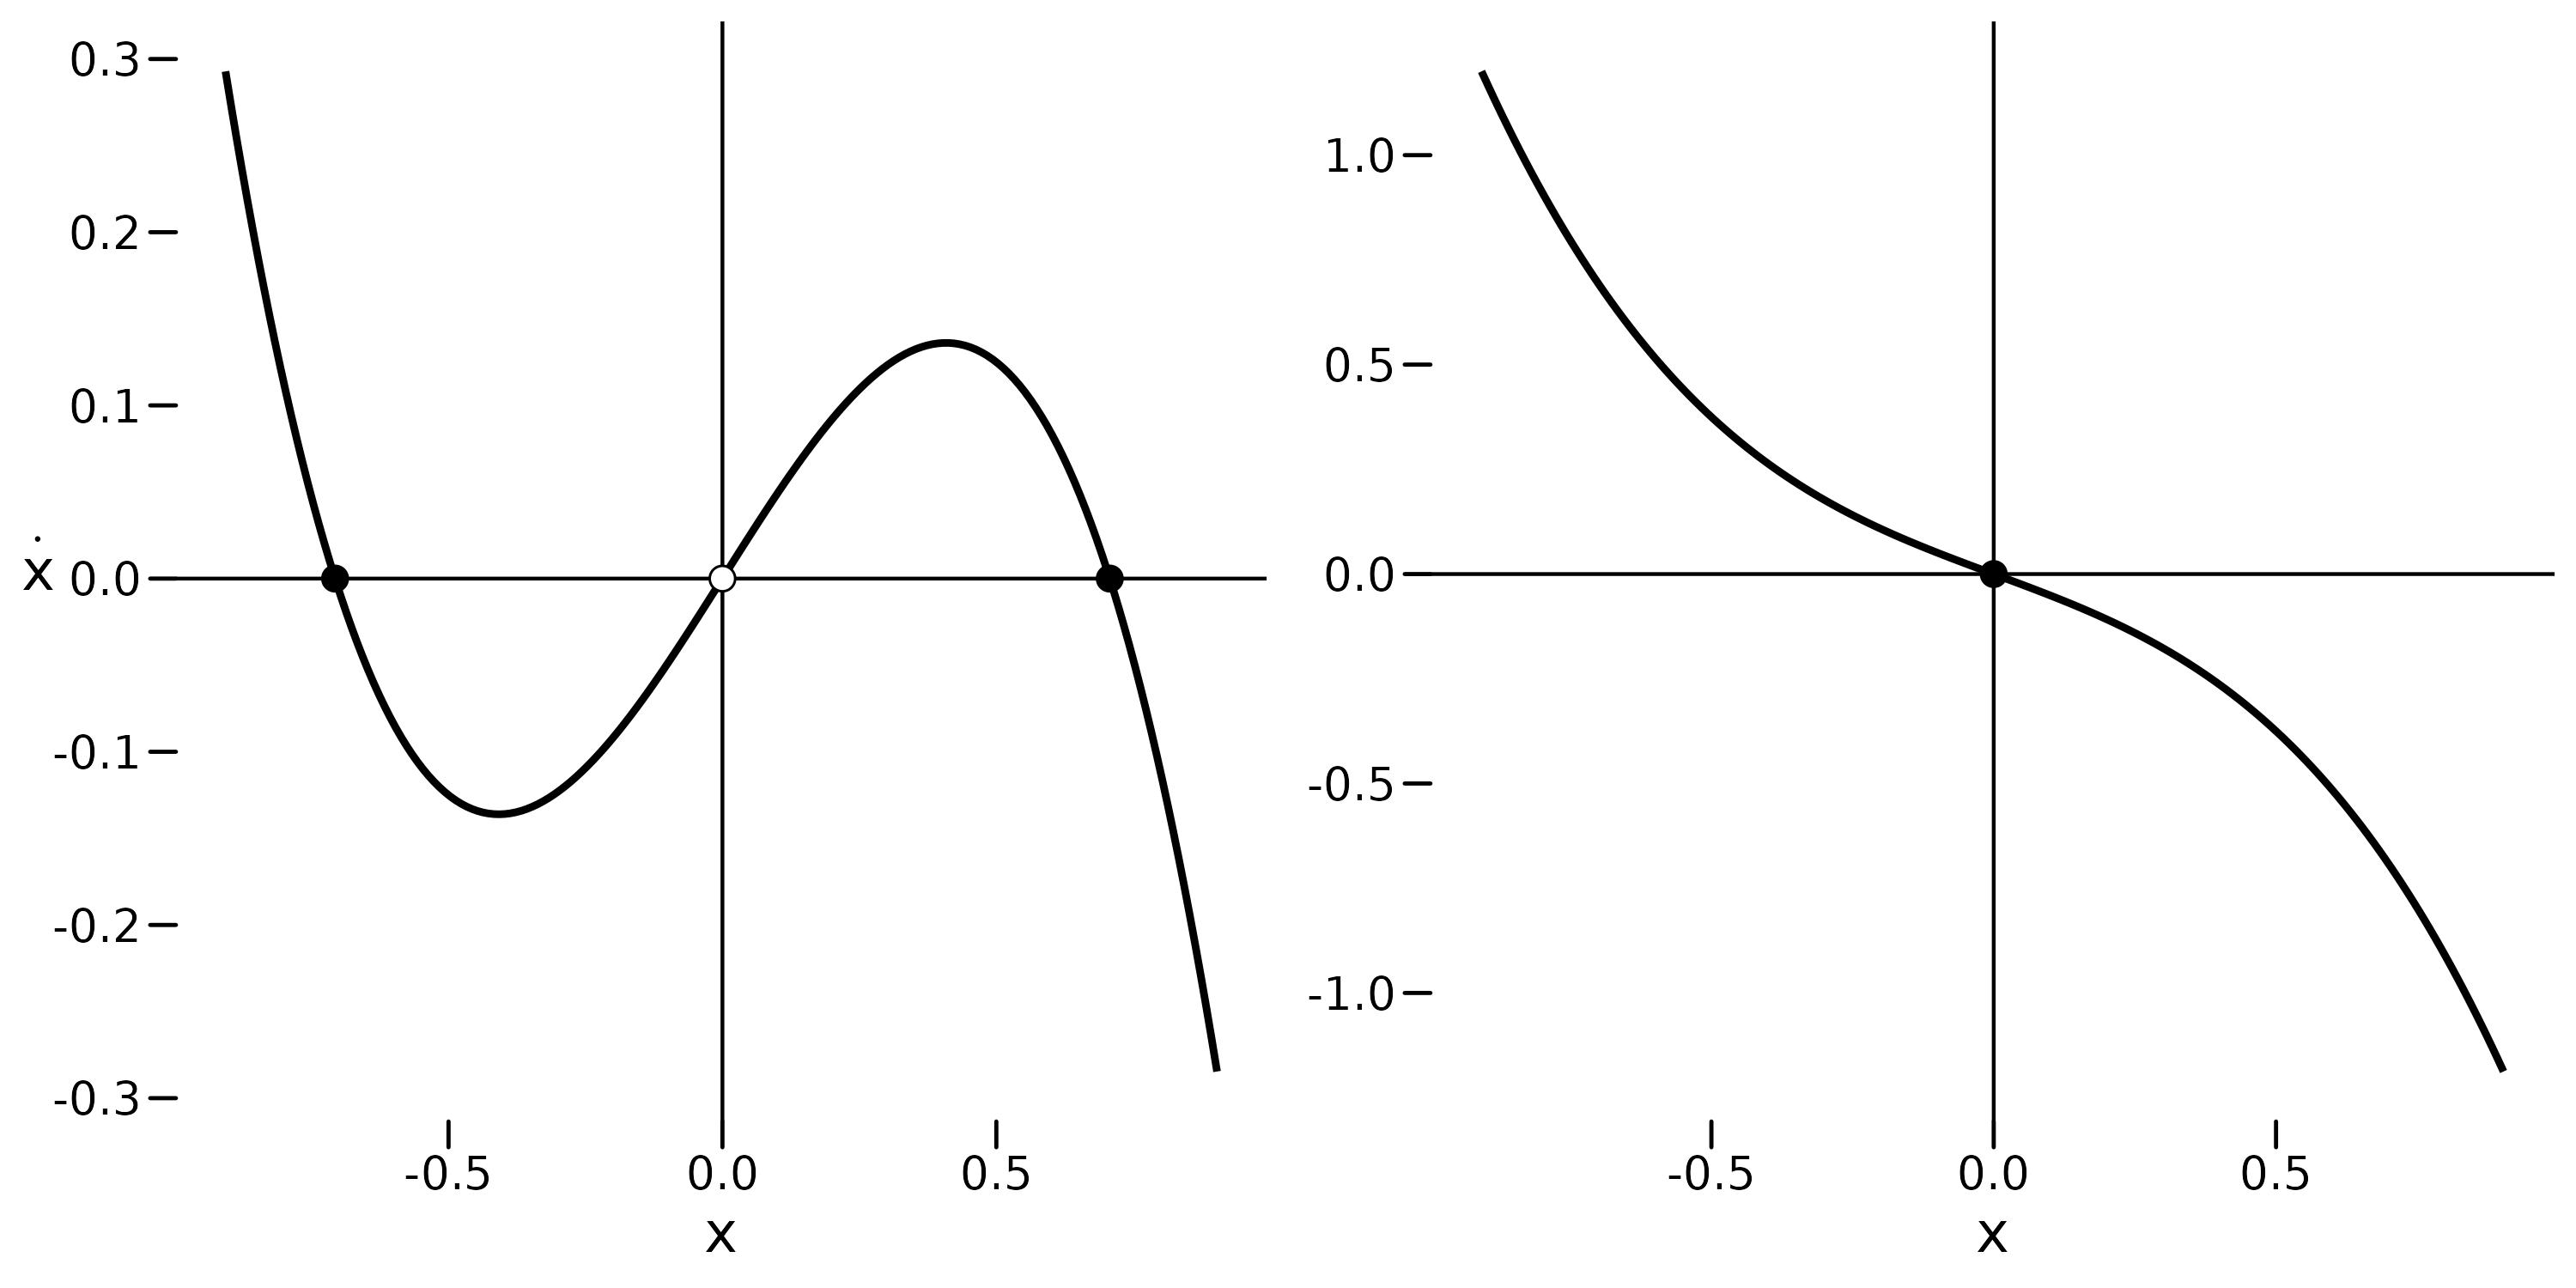
\includegraphics[scale = .125]{figures/double_well_plot_combined.jpeg}
        \caption{The value of the derivative of $X_t$ as a function of $X_t$.
        The graph on the left has $\lambda = -0.5$ and the one on the left has $\lambda = 0.5$.}
    \end{center}
\end{figure}\\
By convention the fixed points are marked by points with stable fixed points being solid points and unstable being hollow and we have fillem them in simply by looking at the graphs. When $\dot{x}_t$ i.e. $x_t'$ is below 0, the flow is to the left and otherwise. In the intercepts we have the fixed points, and by analyzing them in combination with the flow, we get the same results from the plots as we found analytically earlier. \\
The change in behaviour of the systems fixed points $\lambda$ going from negative to positive is a phenomenon that we refer to as bifurcation. What happened was that the fixed points moved closer to one another until they eventually were destroyed for $\lambda > 0$. Depending on the type of bifurcation in question this plays out differently. 
\subsubsection{Saddle-node bifurcation and Tipping Point Estimation}
In the study of dynamical systems, we refer to how changes in parameters affect the qualitative structure of the flow as bifurcations. The parameter values that results in the changes we call bifurcations points. In applications, we sometimes denote these tipping and tipping points, respectively, to get more metaphorical- and intuitive terms. \cite{Strogatz2019_gv}. Nevertheless, we only consider the so-called Saddle-node bifurcations, defined qua the normal form
\begin{align}
    X_t &= \left(\lambda \pm X_t^2\right) \mathrm{d}t \label{standardForm}
\end{align}

The fixed point of the system is always $x^* = \pm\sqrt{\abs{\lambda}}$. There is always one stable- and unstable fixed point. The stable fixed point is the negative branch of the root for the positive version of the normal form, whereas the opposite is true for the negative version. In both cases, the system has its bifurcation point at $\lambda = 0$, where the fixed point becomes half-stable. Lastly, there are no fixed-points for $\lambda>0$ in the positive version of (\ref{standardForm}) and vice versa. Now, in order to make the model more flexible we introduce the parameters, $m, A$ to shift the dynamics and scale the bifurcation point respectively. Then for values of $\lambda$ sufficiently close to the bifurcation point, $\lambda_c = 0$, any system that has the saddle-node bifurcation characteristic is approximated well by 
\begin{align}
    \mathrm{d}X_t &= \pm\left(\lambda + A\left(X_t - m\right)^2\right), 
\end{align}
with $m = \mu \pm \sqrt{\left|\frac{\lambda}{A}\right|}$ and $\mu$ is the stable fixed point of the system. \cite{Ditlevsen2023}. That is, we can be completely agnostic about the overall dynamics of the system. Yet, this naturally implies that we are completely oblivious to them as well. In our applications, the sign of the parameters, $A, \lambda$, will always be different, thus we can simplify the notation in the model to
\begin{align}
    \mathrm{d}X_t &= -\left(A\left(X_t - m\right)^2 + \lambda\right), 
\end{align}
where $m = \mu \pm \sqrt{-\frac{\lambda}{A}}$ the branch corresponds to the sign of $A$. Again, $\mu$ is the stable fixed point of the system. Now, to incorporate uncertainties into the model, we add a noise-term driven by a brownian motion
\begin{align}
    \mathrm{d}X_t &= -\left(A\left(X_t - m\right)^2 + \lambda\right) + \sigma^2(X_t, t)\mathrm{d}W_t, \label{eq:dynamicsOriginal}
\end{align}
where $\sigma^2(X_t, t)$ is a function that dictates how the noise enters the system. This is a stochastic differential equation; for a motivation of this construction see \cite[Chapter 3.1-3.2]{Srkk2019}. Finally, we model the evolution in the dynamics of the system by an extension of \cite[Equation (2)]{Ditlevsen2023}. Namely
\begin{align}
    \lambda_t = \lambda_0\left(1 - \mathds{1}\left(t>t_0\right)\frac{\left(t - t_0\right)}{\tau_c}\right)^\nu \label{eq:lambda_t}.
\end{align}
That is we use the particular form of (\ref{eq:lambda_t}) in (\ref{eq:dynamicsOriginal}). We imagine that our systems exists in some stationary state with $\lambda_t = \lambda_0$ before time $t_0$, after which a ramping starts. Apart from the stochastic part, the model is the saddle-node bifurcation \cite{Strogatz2019_gv}; we study the effects of picking different functions for $\sigma^2(X_t, t)$. More specifically, we consider functions belonging to the class of stochastic differential equations named pearson diffusions. Along with the addition of the $\nu$-parameter, this is an apparent way to extend the model with additive noise presented in \cite[equation (1)]{Ditlevsen2023}. The practical motivations for this class of diffusions will later become clear as we see that the diffusions have readily available tools that allow efficient inference.
\subsection{Inference for stochastic differential equations}
Regardless of ones exact method, inference about parameters in stochastic differential equations are often done by leveraging the markov property of Itô processes. This means that in order to estimate the parameters, it is sufficient to have the transition density or approximations thereof. Getting the transtion density involves solving the Fokker-Planck equation (\ref{eq:fokkerPlanck}). As we mentioned, this is for mostly not possible, thus we employ one or more approximation methods.\\
To this end, inference is traditionally done qua the Euler-maruyama scheme. In this thesis, we only used the estimator based on this scheme in the initial development; it is fairly easy to derive, implement and it is computationally quite efficient. Yet, the estimator is biased even for moderately large stepsizes, and quite notably so in non-linear models \cite{SplittingSchemes}. Instead, we consider two other means of estimation 
\subsubsection{The Strang likelihood}
The Strang based estimator is a method based on splitting schemes. These can also be used to construct the Lie-Trotter based estimator. The common objective of the two methods is to approximate the transition density via the splitting; though, the one-step predictions of transition densities given by the Strang splitting scheme is proven to be superior to the; compare \cite[Proposition 3.4 and 3.6]{SplittingSchemes}, whence we only consider the Strang scheme. We start by looking at the Strang splitting on a general one-dimensional SDE with additive noise. Later we comment on the possible ways to use this method even for models with multiplicative noise.\\
\textbf{Models with additive noise}\\
General one-dimensional stochastic differential equations with additive noise can be written as
\begin{align}
    \mathrm{d}X_t = b(X_t, \theta)\mathrm{d}t + \sigma\mathrm{d}W_t, \label{eq:generalAdditiveNoiseSDE}
\end{align}
note that we have highlighted the dependence of some parameter, $\theta\in\Theta\subseteq\mathbb{R}^p$ in the drift. When we have additive noise, splitting schemes work by decomposing the process into a linear SDE and a non-linear ODE in the following way
\begin{align}
    \mathrm{d}X_t^{(1)} &= -\beta(\theta)\left(X_t^{(1)} - \mu(\theta)\right)\mathrm{d}t + \sigma \mathrm{d}W_t, &&X_t^{(1)} = x_0, \label{SDE_split}\\
    \mathrm{d}X_t^{(2)} &= N\left(X_t^{(2)}; \theta\right)\mathrm{d}t, &&X_t^{(2)} = x_0, \label{ODE_Split}
\end{align}
where $N$ is some non-linear function that probably depends on the parameters. Evidently, this splitting is not unique, and thus the way we construct the estimator will not be either. However, it turns out that any splitting of (\ref{eq:generalAdditiveNoiseSDE}) yields approximations of the transition densities that are equivalent asymptotically \cite{{SplittingSchemes}}. Yet, our choice might still have an impact on the quality of the estimator for finite samples. Additionally, in practice it is not difficult to imagine that some splittings are numerically more well-behaved than others. So we still have to carefully consider our splitting choice. The one we use or the most part is the heuristic provided in \cite[section 2.3 and 2.5]{SplittingSchemes}. That is, (\ref{SDE_split}) should be constructed as the linearization around the fixed points of the drift. This means, we use $b(X_t, \theta)$ from (\ref{eq:generalAdditiveNoiseSDE}) and solve the following equation
\begin{align}
     b(X_t, \theta) = 0,
\end{align}
in terms of $X_t$. $\mu\left(\theta\right)$ is then defined as the solution. This value is plugged into the derivative of $b(X_t, \theta)$ 
\begin{align}
    \beta\left(\theta\right) = \frac{\partial}{\partial x} b(\mu\left(\theta\right), \theta).
\end{align}
The two components, is put together to construct (\ref{SDE_split}).
Hereafter, (\ref{ODE_Split}) is calculated as the residual of the \ref{eq:generalAdditiveNoiseSDE} and our (\ref{SDE_split}). Recall that in the one dimensional case, the solution with stepsize, $\Delta t$, to the linear SDE is given by the flow
\begin{align}
    \varphi_{\Delta t}^{(1)}(x) = \exp\left(-\beta\left(\theta\right) \Delta t\right)\left(x - \mu\left(\theta\right)\right) + \mu\left(\theta\right) + \xi_{\Delta t}, \label{varphiTheoretical}
\end{align}
with $\xi_{\Delta t}\sim\mathcal{N}\left(0, \Omega_{\Delta t}\right)$. That is, the flow is gaussian with mean and variance
\begin{align}
    \mu_{\Delta t}(x; \theta) &= \exp\left(-\beta\left(\theta\right) \Delta t\right)\left(x - \mu\left(\theta\right)\right) + \mu\left(\theta\right) \label{linearSDEMean}\\
    \Omega_{\Delta t} &= \frac{\sigma^2}{2\beta}\left(1 - \exp\left(-2\beta\left(\theta\right)\Delta t\right)\right), \label{linearSDEVariance}
\end{align}
which we calculated in (\ref{eq:OU_solution}). For our purposes the solution to (\ref{ODE_Split}) exists and is unique; this is ensured by the Picard-Lindelöf theorem \cite[section 2.7]{Srkk2019}, since (\ref{ODE_Split}) is ordinary differential equations that in our case will be sufficiently regular for the assumptions from the theorem to hold. Still, a closed form solution to (\ref{ODE_Split}) might not be possible to get, simply due to the complexity of the ODE. In those cases, we will use the Fourth Order Runge-Kutta method to solve it numerically \cite[p.541 equation (8)]{numericalAnalysis}.  
Nevertheless, we denote the solution with stepsize, $\Delta t$, $\varphi_{\Delta t}^{(2)}$. The Strang splitting scheme then gives the approximation of the transition density as 
\begin{align}
    X_{t_{i+1}}^{(S)} = \varphi_{\Delta t / 2}^{(2)}\left(\mu_{\Delta t}\left(\varphi_{\Delta t/2}^{(2)}\left(X_{t_{i}}^{(S)}\right); \theta\right) + \xi_{\Delta t} \; ; \theta \right). \label{eq:classicStrangSplitting}
\end{align}
Due to the fact that (\ref{varphiTheoretical}) is gaussian, (\ref{eq:classicStrangSplitting}) is a non-linear transformation of a gaussian variable; so by the density transformation theorem, the flow gives us the following negative pseudo-loglikelihood 
\begin{align}
    l^{[S]}(\mathbf{X}; \theta) &= -\sum_{i = 0}^{N - 1}\log\left(g\left(\left(\varphi_{\Delta t / 2}^{(2)}\right)^{-1}\left(X_{t_{i+1}}\right); \mu_{\Delta t}\left(\varphi_{\Delta t/2}^{(2)}\left(X_{t_{i}}\right); \theta \right), \Omega_{\Delta t} \right) \right) \nonumber \\
    &- \sum_{i = 0}^{N - 1}\log\left(\frac{\partial}{\partial x}\left(\varphi_{\Delta t / 2}^{(2)}\right)^{-1}\left(X_{t_{i + 1}}\right) \right), \label{Strang_likelihood}
\end{align}
where $N$ is the number of samples. This is the Strang based pseudo-likelihood, and we say that the $\theta$ that minimizes this function is the Strang-based estimator. In (\ref{Strang_likelihood}) $g$ is the density of the gaussian distribution with the specified mean and variance. To get the inverse of the solution to the ODE, we use the property $\left(\varphi_{\Delta t}^{(2)}\right)^{-1} = \left(\varphi_{-\Delta t}^{(2)}\right)$ \cite[Remark below equation (9)]{SplittingSchemes}, and solve ODE corresponding to the right hand side with the Runge-kutta method. Finally, to get the derivative we use Richardson extrapolation. For a function, $f$, the derivative can be approximated as
\begin{align}
    f'(x) = \frac{f(x + h) - f(x - h)}{2h}, \qquad h > 0,
\end{align}
with an error that is $\mathcal{O}(h^2)$. It is possible to repeatedly use Richardson extrapolation to get even higher-orders of precision. However, for our purposes this simple approximation suffices.
\\\\
\textbf{Models with multiplicative noise}\\
As we noted, we require additive noise in the models. This is, because the method hinges on that we an Ornstein-Uhlenbeck process in (\ref{SDE_split}). For many models that interest us, this, of course, not be the case in itself. But all the models we consider are reducible, and as such we can transform the processes with the lamperti-transform (\ref{eq:lampertiDefinition}) and do the estimation on the resulting SDE in the exact manner as we just described. This is the method introduced in \cite{SplittingSchemes}, for which there exist theoretical results on the accuracy of the transition density.\\
Still, we consider different options. As an alternative, we use the same splitting philosophy, but leave the noise as it is. This of course means that the linear SDE inherits the multiplicative noise. Other methods for approximating such methods exist. The one we use is Kessler's method; this method assumes a gaussian transition density, but uses the true conditional mean- and variance \cite[equation (1.7)]{Kessler1997}. Even still, there is another possibility. In a few cases there exists other closed form solutions to linear stochastic differential equations than the one with additive noise. This splitting strategy avoids using the Lamperti-transform, while avoiding approximating any solution to an SDE. Although, the last two types of splittings are not central to the thesis, we still illustrate. Derivation for the latter option can for instance be seen in (\ref{meanrevertingGBMSplit1}). Note that in this example, we must use a different splitting than the heuristic provided by \cite[section 2.3 and 2.5]{SplittingSchemes}, because the solution of the stochastic differential equation in the example only exists on closed-form, whenever $\mu(\lambda) = 0$. We would have to be quite fortunate to have the fixed point equal 0; thus this splitting strategy rarely aligns with the heuristic from the paper.
\subsubsection{Approximately Optimal Martingale Estimation Equations}\label{subsubsec:approximatelyOptimalMartingaleEstimationEquation}
Other than the strang splitting, we also estimate the parameters by means of approximately optimal martingale estimation functions (AOMEF). As a means of estimation these are conceptually different from what we have done thus far; with them our aim is not to approximate the transition density, but instead construct functions where the estimator is defined as a solution to a system of equations similarly to how a score function (\ref{eq:transitionScore}) normally is used.\\ Not surprisingly, AOMEF's are based on the notion of a martingale estimaton equation. To construct a general martingale estimation function, we imagine that we want to estimate some parameter, $\theta\in \Theta \subseteq \mathbb{R}^p$, in a one-dimensional stochastic differential equation such as (\ref{eq:firstSDE}); and say that the solution to this equation has state space, $D\subseteq \mathbb{R}$. Furthermore, let $p(x, y, \Delta t; \theta)$ be the transition density of $X_{t+\Delta t}$ given $X_t$, evaluated at the point $y$. Then a martingale estimation function is 
\begin{align}
    G_N(\theta) = \sum_{i = 1}^N g(X_{t_{i - 1}}, X_{t_i}, \Delta t; \theta), \label{eq:estimationEquation}
\end{align}
where $g$ is some function such that
\begin{align}
    \int_{D} g(x, y, \Delta t; \theta)p(x, y, \Delta t; \theta)\mathrm{d}y = 0. \label{eq:martingaleProperty}
\end{align}
In other words, $G_N$ is a martingale w.r.t. the filtration $\mathcal{F}_n = \sigma\left(X_{t_i}; i \leq n\right)$. \cite[p. 11]{StatisticalMethodsForSDE} establishes that an example of such an equation are the score equations; this is easily seen by inserting (\ref{eq:transitionScore}) in (\ref{eq:martingaleProperty}). That is the martingale equations can be seen as a generalization of the score equation. Now, we know that the solving the score equation yields the maximum likelihood estimator; an estimator with many desirable properties. Thus, we are interested in picking a function $g$ satisfying (\ref{eq:martingaleProperty}) that is optimal in the sense that it approximates the score well. We do this by taking a collection of real valued functions $h = (h_1, \dots, h_m)^\top$, where each individual function satisfies (\ref{eq:martingaleProperty}) and choose $g$ in (\ref{eq:estimationEquation}) so
\begin{align}
    G_N(\theta) = \sum_{i = 1}^N a\left(X_{t_i}, \Delta t, \theta \right)h(X_{t_{i - 1}}, X_{t_i}, \Delta t; \theta), \label{eq:estimationEquationWeight},
\end{align}
where $a$ is a $p\times m$-matrix that is a function that (\ref{eq:estimationEquationWeight}) is integrable w.r.t. $P_\theta$. Therefore (\ref{eq:estimationEquationWeight}) is a martingale, because the $h_j$ satisfy (\ref{eq:estimationEquation}). The $h$-functions are often chosen such that
\begin{align}
    h_j = f_j(X_i, \Delta t) - \mathbb{E}_\theta\left[f_j(X_i)| X_{t_{i - 1}} = x_{t_{i - 1}}\right]
\end{align}

(MANGLER NOGET HER - HVOR MEGET SKAL DER MED?)


\begin{align}
    G_N^{\circ} &= \sum_{i = 1}^N 
    \left(
        \frac{\partial_\theta b\left(X_{t_{i-1}};\theta\right)}{\sigma^2\left(X_{t_{i-1}};\theta\right)}
    \right) \left(X_{t_{i}} - \mathbb{E}\left[X_{t_{i}} \middle| X_{t_{i-1}} = x\right]\right) \nonumber \\
    &+ \frac{\partial_\theta\sigma^2\left(X_{t_{i-1}}; \theta\right)}{2\sigma^4\left(X_{t_{i - 1}}; \theta\right)\Delta t}\left(\left(X_{t_{i}} - \mathbb{E}\left[X_{t_{i}} \middle| X_{t_{i-1}} = x\right]\right)^2 - \textrm{Var}\left[X_{t_{i}} \middle| X_{t_{i-1}} = x\right]\right) \label{eq:approximatelyOptimalMartingale}
\end{align}
\cite[Example 1.11]{StatisticalMethodsForSDE}.

\subsection{Numerical Optimization in \code{R}}
Numeric optimization is central in applications of machine learning and statistics. In this section, we mention the methods used in the thesis and some motivation for the choices that was made. Also, we introduce a numerical Strang-based negative log-likelihood based on the heuristics of \cite{SplittingSchemes}, where the user only needs to specify the drift of the lamperti-transformed SDE.
\subsubsection{General optimization and implementation}
For each part of the process i.e. before and after ramping begins, we optimize a bit differently. Because of this, we have implemented two wrappers around {stats::optim} \cite{Rlang}. Of course, the wrapper that optimizes the process before ramping begins can be called with any likelihood function, we have implemented for that part; the same also holds true for the dynamic part. In addtion, we allow any valid \code{optim}-argument as required to be called in both wrappers; the is especially useful, because the arguments to \code{optim} can vary depending on the specific algorithm, one wishes to use. Also, since \code{optim} uses an ellipsis, our wrappers does too. That is, our wrapper can pass on any argument directly onto \code{optim}. This is for example useful, if we have objective functions with different inputs.\\
Still, the wrapper obviously has to have a couple of default arguments in the invokation to make easier to use. For instance, both parts use the built-in BFGS optimization algorithm, due to its robustness; though, as said we could specify any other optimization algorithm implemented in \code{optim} during the call.\\ For the dynamic part, we need to provide the values for $\alpha_0, \mu_0, \sigma$. This the ellipsis seemingly allows us to do. Of course, the values we pass on here are the estimated values for these from the stationary part of the processes. In addition, the optimizer of the dynamic part dynamically chooses to estimate the $\nu$-parameter dependending on the dimension of the initial values that are provide to it. If the dimension is two, we implicitly assume $\nu = 1$, while a dimension of three allows the optimizer to estimate it. With regards to the numerical stability of the implementations we do a few things. Firstly, terms including $\exp\left(x\right) - 1$ or its additive inverse show up in many of our formulas. This is for instance the case in (\ref{linearSDEVariance}). As the arguments for the exponential function often is quite close to zero in these applications, we need to take care in order to avoid catastrophic cancellation. Luckily, others have had this problem before us, and we make use of the \code{base::expm1} method in \code{R}, which calls the C-function of the same name \cite{cppreference_expm1} - a method optimized for this very problem. If we do not do this, our program might crash or give misleading estimates. In the case of (\ref{linearSDEVariance}) for instance, we risk having a variance of zero. While the methods in \code{R} that use the gaussian distribution allow the use of this degenerate distribution, we are of course not interested in such a transition density.
\subsubsection{A numerical Strang method in \code{R}}
In this section, we briefly describe an almost entirely numerical Strang splitting scheme based estimator with our usual splitting philosophy. The algebra required in the derivations of this method to obtain the necessary elements can be quite cumbersome. We have already limited the amount of errors we can do somewhat by relying on the Fourth-Order Runge-kutta method to solve ODE's in some of the versions of the Strang splitting. Limiting the amount of computations further could have an advantage; however it is naturally more difficult to implement. Nevertheless, As of the current implementation, we are at the amount of automation, we we only need to derive two things ourselves: The Lamperti-transform and the drift of the SDE that comes as a result of it. Passing these onto our wrapper for the optimizer and we optimize the Strang-based likelihood. \\
The method works the same as the less automated versions with regards to solving the ODE's. However, the construction of (\ref{SDE_split}) and (\ref{ODE_Split}) is different. The latter is of course just computed as the residual of lampert transformed drift that we pass to the method and the linear SDE. The linear SDE is constructed as the linearization around the fixed point of the drift. The fixed point is found using the method \code{nleqslv::nleqslv}, which find zeroes with Newton's method \cite{nleqslv}. We then find the derivative of the drift numerically with \code{numDeriv::grad} \cite{numDeriv}. We plug the fixed point into this function to get the the slope of the linearization.
\subsection{Model assessment}
For this part, we briefly introduce the metrics used for evaluating the quality of our estimators in a simulation setting. Additionally, we show the method that we use to diagnose the fit of a particular method to data, and how we contruct confidence intervals for the estimators.
\subsubsection{Diagnostics and confidence intervals}
When we are in a simulation setting, we assess the precision of our estimation methods using the mean of the absolute relative error over a number of simulations, $M$, each with sample size, $N$. This is for the $i$th-coordinate in our parameter vector defined as
\begin{align}
    \mathrm{ARE}\left(\theta_N^{(i)}\right) = \frac{1}{M}\sum_{j = 1}^M\frac{\left|\theta_{N,j}^{(i)} - \theta_{0,j}^{(i)}\right|}{\theta_{0,j}^{(i)}}.
\end{align}
Of course, we are not able to calculate this quantity when we do not have access to the ground-truth parameters. Also, we cannot use regular residuals to diagnose the fit, as each data point have different distributions depending on the previous point. Instead, we assess the fit qua so-called uniform residuals. These are constructed using the transition density, $p_\theta(x|\Delta t, x_0)$. Though, as is quite clear by now, this is rarely something we can compute. However, we can use the approximation given from the Strang scheme in its stead. This also gives us an approximation for the conditional distribution function, $F_\theta(x|\Delta t, x_0)$, and as $F_\theta(X_{t_{i}}|\Delta t, X_{t_{i - 1}})\sim \mathrm{Unif}(0,1)$ if $X_{t_{i}}|X_{t_{i - 1}} \sim p_\theta$. It is sometimes difficult to detect outliers in the uniform distribution, so we transform the quantity with the quantile function of the standard gaussian distribution, such that we by the quantile transformation theorem have samples that are standard gaussian. The fit can then be diagnosed by means of ordinary Q-Q plots.\\
As the approximately optimal martingale estimation functions approximate the score function, we do not have any approximation of the transition density here and cannot use uniform residuals. Even still with some creativity, we can do diagnostics, but only of the square-root process. If we let $X_t$ to be governed by the square-root process, then
\begin{align}
    Y_{t_{i + 1}} := \frac{4\beta}{\sigma^2\left(\exp\left(-\beta \Delta t\right) - 1\right)}X_{t_{i + 1}}
\end{align}
has transition density of a non-central $\chi^2$-distribution with $\frac{4\beta\mu}{\sigma^2}$ degrees of freedom with non-centrality parameter $Y_{t_k}\exp\left(-\beta \Delta t\right)$ \cite[Equation (5.68)]{Srkk2019}. For the other diffusions, we do not have an analagous property to exploit, and we may only assess the score function based estimators by ensuring that the estimates are consitent with methods based on the transition density; for which we use the uniform residuals. Finally, we obviously have no hope of knowing the distribution of our estimators. Therefore to get an idea of our uncertainty of them, we use parametric bootstrap. That is, we estimate on the data with a specific model and then sample from that model repeatedly using the parameters estimated on the real data. The empiric distribution of the estimates achieved in this way then gives us the quantiles etc. for our estimator.